%%{ DOC HEAD

\pdfoutput=1
\documentclass[a4paper,11pt,titlepage,twoside]{book}

\usepackage[english]{babel}
\usepackage[utf8]{inputenc}
\usepackage{amssymb,amsmath}
\usepackage{algorithm,algpseudocode}
\usepackage[title,titletoc]{appendix}
\usepackage{latexsym}
\usepackage{a4wide}
\usepackage{color}
\usepackage{indentfirst}
\usepackage{graphicx}       %%% graphics for dvips
\usepackage{fancyhdr, lastpage}
\usepackage{longtable}
\usepackage{pifont}
\usepackage{makeidx}
\usepackage{multirow}
\usepackage{dcolumn}
\usepackage{epstopdf}
\usepackage{url}
\usepackage{listings}
\usepackage{caption}
\usepackage{subcaption}
\usepackage{relsize}
\usepackage{pdfpages}
\usepackage{url}
\usepackage{lipsum}
\usepackage{isotope}

\usepackage{tikz}
\usetikzlibrary{shapes.arrows,backgrounds,arrows,automata,shapes,positioning,calc,through}

%%{ ARROWS

\tikzset{
  myarrow/.style={
    draw,
    fill=orange,
    single arrow,
    minimum height=3.5ex,
    single arrow head extend=1ex
  }
}

\newcommand{\arrowup}{%
  \vspace{-0.8em}
  \tikz [baseline=-0.5ex]{\node [myarrow,rotate=90] {};}
  \vspace{-1.4em}
}

\newcommand{\arrowdown}{%
  \vspace{-0.8em}
  \tikz [baseline=-1ex]{\node [myarrow,rotate=-90] {};}
  \vspace{-1.5em}
}

\newcommand{\arrowright}{%
  \tikz [baseline=-1ex]{\node [myarrow,rotate=0] {};}
}

\newcommand{\arrowleft}{%
  \tikz [baseline=-1ex]{\node [myarrow,rotate=180] {};}
}

%%}

%%{ CHECKMARK

\def\checkmark{\tikz\fill[scale=0.4](0,.35) -- (.25,0) -- (1,.7) -- (.25,.15) -- cycle;}

%%}

\pgfdeclarelayer{background}
\pgfdeclarelayer{foreground}
\pgfsetlayers{background,main,foreground}

\tikzset{
  state/.style={
    rectangle,
    draw=black, very thick,
    minimum height=1.0em,
    text centered,
  },
  state_gray/.style={
    rectangle,
    draw=black, very thick,
    fill=gray!40,
    minimum height=1.0em,
    text centered,
  },
  state_white/.style={
    rectangle,
    draw=black, very thick,
    fill=white,
    minimum height=1.0em,
    text centered,
    text=black,
  },
  state_green/.style={
    rectangle,
    draw=black, very thick,
    fill=green!50,
    minimum height=1.0em,
    text centered,
    text=black,
  },
  state_red/.style={
    rectangle,
    draw=black, very thick,
    fill=red!70,
    minimum height=1.0em,
    text centered,
    text=black,
  },
  state_blue/.style={
    rectangle,
    draw=black, very thick,
    fill=blue!40,
    minimum height=1.0em,
    text centered,
    text=black,
  },
  final_state/.style={
    rectangle,
    rounded corners,
    draw=black, very thick,
    minimum height=2em,
    text centered,
  },
  initial_state/.style={
    rectangle,
    double=white,
    double distance=1pt,
    inner sep=2pt,
    draw=black, very thick,
    minimum height=2em,
    text centered,
  },
  point/.style={
    circle,
    inner sep=0pt,
    minimum size=3pt,
    fill=red
  },
}



% change formatting of lists
\usepackage{enumitem}
\setlist{nosep}
% \setlist{noitemsep}
% how to format particular lists?
% \begin{itemize}[topsep=8pt,itemsep=4pt,partopsep=4pt, parsep=4pt]

% change spacing of the table of contents
\usepackage{tocloft}
% \renewcommand\cftchapafterpnum{\vskip5pt}
% \renewcommand\cftsecafterpnum{\vskip5pt}

% change formatting of a chapter
\usepackage{titlesec}
\titleformat{\chapter}[block]
{\normalfont\huge\bfseries}{Chapter \thechapter\\\vspace{0.1em}\\}{1em}{\Huge}
% {?}{before}{after}
\titlespacing*{\chapter}{0pt}{-1em}{2em}

%%{ BIBLATEX

\usepackage[backend=bibtex,defernumbers=true,style=ieee]{biblatex}

\newcommand{\Font}{\fontfamily{cmr}\selectfont} % classical latex font
\renewcommand*{\bibfont}{\Font}
\newcounter{bbx:primcount}
\setcounter{bbx:primcount}{0}

\newcounter{bbx:allcount}
\setcounter{bbx:allcount}{0}

% Print labelnumbers with suffixes, adjust secondary labelnumber 1/2 (start new numbering of my publications)
\makeatletter
\AtDataInput{%
  \ifkeyword{mine}
  {\addtocounter{bbx:allcount}{1}}%
  {\addtocounter{bbx:primcount}{1}%
    \blx@setlabwidth{\labelnumberwidth}{%
\csuse{abx@ffd@*@labelnumberwidth}{\thefield{labelnumber}a}}}}
\makeatother

% Print labelnumbers with suffixes, adjust secondary labelnumber 2/2
\DeclareFieldFormat{labelnumber}{%
  \ifkeyword{mine}
  {{\number\numexpr#1-\value{bbx:primcount}}a}
{#1}}}

\addbibresource{bib_postprocessed.bib}

\defbibenvironment{favoritebib}
{\itemize}
{\enditemize}
{\item}

%%}

%%{ CUSTOM MACROS

\newcommand{\unit}[2]{$#1~\ensuremath{\mathrm{#2}}$}
\newcommand{\strong}[1]{\textbf{#1}}
\newcommand{\coord}[1]{\textbf{#1}}
\newcommand{\norm}[1]{\left\lvert#1\right\rvert}
\newcommand{\m}[1]{\ensuremath{\mathbf{#1}}}
\newcommand\numberthis{\addtocounter{equation}{1}\tag{\theequation}}
\newcommand{\corrected}[1]{{\color{black} {#1}}}
\newcommand{\updated}[1]{{\color{black} {#1}}}

\newcommand{\conditionalClearPage}{
  \ifdefined\printversion
  %\newpage{}
  %\thispagestyle{empty}
  \clearemptydoublepage
  %\cleardoublepage{\thispagestyle{empty}}
  \else
  \newpage{}
  \clearpage
\fi
}

%%}

\newcommand{\Author}{Ing. Tomáš Báča}
\newcommand{\Supervisor}{Ing. Martin Saska, Dr. rer. nat.}
\newcommand{\Specialist}{Ing. Michal Platkevic, Ph.D.}
\newcommand{\Programme}{Electrical Engineering and Information Technology}
\newcommand{\Field}{Artificial Intelligence and Biocybernetics}
\newcommand{\Title}{Cooperative Sensing with Group of Unmanned Aerial Vehicles}
\newcommand{\DocName}{Doctoral Thesis}
\newcommand{\Keywords}{Unmanned Aerial Vehicles, Ionizing localization}
\newcommand{\Date}{1/1/2019}
\newcommand{\DOCVersion}{0.1}

% % altering margins
% \setlength{\oddsidemargin}{+0.5cm}
% \setlength{\evensidemargin}{-0.5cm}

% ??
\def\clinks{false}

% listings
\lstset{breaklines=true,captionpos=b,frame=single,language=sh,float=h}
\lstloadlanguages{sh,c}
\def\lstlistingname{Listing}
\def\lstlistlistingname{Listings}

% European layout (no extra space after `.')
\frenchspacing

% no indent, free space between paragraphs
\setlength{\parindent}{1cm}
\setlength{\parskip}{1ex plus 0.5ex minus 0.2ex}

% offsets the head down
\setlength{\headheight}{18pt}

% foot line
\renewcommand{\footrulewidth}{0.4pt}

\fancypagestyle{plain}

% clear the default layout
\fancyhead{}
\fancyfoot{}

% page header
\fancyhead[LO]{\leftmark}
\fancyhead[RE]{\rightmark}
\fancyhead[LE,RO]{\thepage/\pageref{LastPage}}

% page footer
\fancyfoot[L]{CTU in Prague}
\fancyfoot[R]{Department of Cybernetics}
\fancyfoot[C]{}

\begin{document}

\begin{titlepage}
\begin{center}

{\Large CZECH TECHNICAL UNIVERSITY IN PRAGUE}
\vskip 10pt

\vskip 8pt
{\Large Faculty of Electrical Engineering}
 
%\vskip 0pt plus 2fill
\vspace{50pt}
{\Huge\bf DISSERTATION THESIS}\\
\vspace{40pt}

\includegraphics[width=10cm]{fig/lev.pdf}

\vspace{40pt}
{\Large\rm \Author } \\
\vspace{20pt}
{\Large\bf \Title}

\vspace{60pt}
{\bf Department of Cybernetics}\\
\vspace{5pt}   
{Thesis supervisor: {\bf \Supervisor}}

\vspace{30pt}
%{\sc Prague 2013}
\end{center}
\end{titlepage}


\pagestyle{fancy}

\tableofcontents

%%}

\cleardoublepage

%% --------------------------------------------------------------
%% |                  Chapter 1 - Introduction                  |
%% --------------------------------------------------------------

\chapter{Introduction}

%%{ Introduction

Before remotely controlled and autonomous mobile robots become available, human presence was required for any in situ measurement.
Be it at the bottom of a sea or outside of the Earth's atmosphere, sensing in unreachable places was impossible.
Nowadays, terrestrial sensing is not short on utilizing robotic platforms in hazardous environments.
Since the widespread of Unmanned Aerial Vehicles (UAVs), often called \textit{drones}, much effort was directed towards creating flying platforms capable of sensing the environment \cite{pajares2015overview}.
Aircraft can traverse ground obstacles and move quickly to the desired location when compared to ground robots.
Although, the presented system is designed for use with any mobile platform, including even satellites, where it was successfully deployed \cite{baca2018vzlusat, baca2018rospix}, let us put this paper into the context of MAVs, with their highest applicability,

Micro Aerial Vehicles (MAVs) are small UAVs which can be handled by a single person.
Multirotor helicopters are popular MAVs due to their simple construction and low maintenance.
As the technology of small and intelligent aircraft became available, many fields started to utilize new options for carrying sensor equipment.
Security and rescue forces utilize camera equipment and often thermal imaging cameras to assist ground forces during environmental disasters like earthquakes and floods \cite{yuan2015survey, perks2016advances}.
In research and science, unmanned aircraft have various roles, from testbeds for control algorithms to autonomous sensor carriers.
This paper will focus on a novel sensor setups for autonomous ionizing radiation mapping and localization by UAVs.

Demand for UAV platforms capable of localizing an unknown radiation source is increasing.
Early attempts to design a radiation detection module for a UAV was presented in \cite{kurvinen2005design}.
Fixed-wing aircraft, equipped with Kromek \unit{1}{cm^3} gamma-ray spectrometer, was used to scan legacy mines in England \cite{martin2015use}.
Area of the size of \unit{300}{m} $\times$ \unit{400}{m} was covered during the total of 5 hours of flight, and a radiation map was created ex-post.
A solution suited for a search for compact sources of radiation was presented in \cite{pollanen2009radiation, pollanen2009performance}.
The system utilizes \unit{5}{cm^3} scintillator with an air sampler, which takes measurement of \textit{counts per second} in \unit{1}{s} intervals.
Authors tested that the aircraft can detect presence of \isotope[137]{Cs} (activity \unit{2.3}{GBq}) and \isotope[60]{Co} (activity \unit{1.1}{GBq}) from a distance up to \unit{50}{m}, while flying at \unit{70}{km/h}.
The plane followed a path designed by a human operator.
Another remotely controlled aircraft system is proposed in \cite{aleotti2015unmanned}.

Since Fukushima Daiichi nuclear power plant (FDNPP) incident, research groups aim to prepare aircraft, that would remotely scan the affected area without endangering human workers \cite{macfarlane2014lightweight, martin20163d, martin2015use, sanada2015aerial, tang2016efficiency, towler2012radiation, han2013lowcost}.
Authors of \cite{tang2016efficiency} present an aerial solution equipped with two gamma-ray spectrometers.
Data would be transmitted to a ground station over a data link during the flight.
In \cite{han2013lowcost} a multi-UAV approach was taken to enhance the potential yield of information gain from onboard sensors.
Three formation types and trajectory schemes for three fixed-wing aircraft are proposed in a scenario with simulated sensor scanning.
A multirotor MAV was used in \cite{macfarlane2014lightweight} to carry lightweight CdZnTe \textit{Kromek} spectrometer with \unit{1}{cm^3} of detection material.
Real-world experiments, situated in \unit{20}{m^2} area, showed a process of creating a radiation map where several uranium samples were located.
During the flight, the unmanned vehicle followed a flight plan with a set of waypoints.
Scanning of \unit{1}{km^2} area was also conducted using the \textit{Kromek} detector, near FDNPP \cite{martin20163d, martin2015use}.
The fixed-wing plane carried a laser rangefinder, which was later used to create a 3-D map of the radiation above the affected area.
The plane was controlled remotely or flew according to a pre-fabricated flight plan.

A multitude of published work relies on Kromek spectrometer, which measures the \textit{counts per second}, i.e., the number of ionizing particles that interacted with the detector \cite{han2013lowcost, macfarlane2014lightweight, martin20163d, martin2015use}.
Others use scintillating detectors \cite{sanada2015aerial, towler2012radiation}.
Scintillators are large and heavy, compared to other sensors, and require a large aircraft.
A \unit{94}{kg} UAV conducted flights around FDNPP \cite{sanada2015aerial} and a radiation map of the area was estimated.
The UAV was flying a preprogrammed path through waypoints.
The only exhibit of an algorithmic approach to locating an unknown radiation source in real-time was presented in \cite{towler2012radiation}.

\section{Motivation \& thesis goals}

\section{Thesis contributions}

\section{Mathematical notation and nomenclature}

%%{ mathematical notation

The table \ref{tab:notation} denotes the mathematical notation used throughout this thesis.

\begin{table}[h]
  \centering
  \begin{tabular}{ll}
    \hline
    Symbol & Description \\
    \hline
    lower or uppercase letter, e.g., $n$, $N$ & a scalar \\
    bold lowercase letter, e.g., \textbf{x} & a column vector \\
    bold uppercase letter, e.g., \textbf{A} & a matrix \\
    $\textbf{x}^T$, $\textbf{A}^T$ & vector and matrix transpose \\
    underlined vector, e.g., \textbf{\underline{x}} & concatenated vectors $\left[\textbf{x}_1^T,\textbf{x}_2^T,...,\textbf{x}_n^T\right]^T$ \\
    \textbf{I} & identity matrix \\
    \textbf{1} & unity matrix \\
    $x^{(W)}$ & $x$ in coordinate system $W$ \\
    $x_{[n]}$, $\textbf{x}_{[n]}$ & $x$, $\textbf{x}$ in the sample time $n \in \mathbb{N}$ \\
    $\mathbb{R}$, $\mathbb{N}$ & set of real and natural numbers \\
    \hline
  \end{tabular}
  \caption{Overview of mathematical notation.}
  \label{tab:notation}
\end{table}

%%}

%%}

%% --------------------------------------------------------------
%% |                  Chapter 2 - Related work                  |
%% --------------------------------------------------------------

\chapter{Background and related work}

%%{ Related work

\section{Micro Aerial Vehicles}

\subsection{Control inputs}

\subsection{Multirotor dynamics}

\subsection{Automatic control}

\subsection{Frame of reference conventions and nomenclature}

\section{Target following with an MAV}

\section{Ionizing radiation localization}

\subsection{Radiation detection principles}

\subsection{Detector types}

\subsection{Pixel detectors}

\section{Radiation localization by aerial vehicles}

%%}

%% --------------------------------------------------------------
%% |              Chapter 3 - Micro Aerial Vehicles             |
%% --------------------------------------------------------------
%% |                   MMAR 2016 Embedded MPC                   |
%% |                    IROS 2018 MPC Tracker                   |
%% --------------------------------------------------------------

\chapter{Micro Aerial Vehicles}

%%{ Micro Aerial Vehicles

\section{Multirotor helicopter model}

\subsection{Rotational dynamics}

\subsection{Translational dynamics}

\subsection{Propulsion model}

\section{Agile trajectory tracking with MAV collision avoidance}

\section{Robust hybrid nonlinear predictive controller}

%%}

%% --------------------------------------------------------------
%% |                  Chapter 4 - MRS Platform                  |
%% --------------------------------------------------------------

\chapter{Research-focused MAV platform}

%%{ MRS platform

\section{Paradigms for research and evaluation}

\section{System's building blocks}

\section{Control system architecture}

\begin{figure}
  \pgfdeclarelayer{foreground}
\pgfsetlayers{background,main,foreground}

\tikzset{radiation/.style={{decorate,decoration={expanding waves,angle=90,segment length=0.1em}}}}

\begin{tikzpicture}[->,>=stealth', node distance=7.0em]

  \node[state_blue, shift = {(0.0em, 0.0em)}] (uav_manager) {
    \begin{tabular}{c}
      \small UAV manager
    \end{tabular}
  };

  \node[state_blue, below of = uav_manager, shift = {(0.0em, -0.0em)}] (control_manager) {
    \begin{tabular}{c}
      \small Control manager
    \end{tabular}
  };

  \node[state_red, right of = control_manager, shift = {(5.0em, 0.0em)}] (landoff_tracker) {
    \begin{tabular}{c}
      \small Landoff Tracker
    \end{tabular}
  };

  \node[state_red, below of = landoff_tracker, shift = {(0.0em, 4.5em)}] (mpc_tracker) {
    \begin{tabular}{c}
      \small MPC tracker
    \end{tabular}
  };

  \node[state_red, below of = mpc_tracker, shift = {(0.0em, 4.5em)}] (joy_tracker) {
    \begin{tabular}{c}
      \small Joy Tracker
    \end{tabular}
  };

  \node[state_red, below of = joy_tracker, shift = {(0.0em, 4.5em)}] (matlab_tracker) {
    \begin{tabular}{c}
      \small Matlab Tracker
    \end{tabular}
  };

  \node[state_red, below of = matlab_tracker, shift = {(0.0em, 4.5em)}] (csv_tracker) {
    \begin{tabular}{c}
      \small CSV tracker
    \end{tabular}
  };

  \node[state_green, left of = control_manager, shift = {(-5.0em, 0.0em)}] (so3_controller) {
    \begin{tabular}{c}
      \small SO(3) controller
    \end{tabular}
  };

  \node[state_green, below of = so3_controller, shift = {(0.0em, 4.5em)}] (mpc_controller) {
    \begin{tabular}{c}
      \small MPC controller
    \end{tabular}
  };

  \node[state_blue, above of = so3_controller, shift = {(0.0em, -2.0em)}] (gain_manager) {
    \begin{tabular}{c}
      \small Gain manager
    \end{tabular}
  };

  \node[state_green, below of = mpc_controller, shift = {(0.0em, 4.5em)}] (failsafe_controller) {
    \begin{tabular}{c}
      \small Failsafe controller
    \end{tabular}
  };

  \node[state_green, below of = failsafe_controller, shift = {(0.0em, 4.5em)}] (nsf_controller) {
    \begin{tabular}{c}
      \small NSF conroller
    \end{tabular}
  };

  \node[state_green, below of = nsf_controller, shift = {(0.0em, 4.5em)}] (attitude_controller) {
    \begin{tabular}{c}
      \small Attitude controller
    \end{tabular}
  };

  \node[state_blue, above of = landoff_tracker, shift = {(0.0em, -2.0em)}] (constraint_manager) {
    \begin{tabular}{c}
      \small Constraint manager
    \end{tabular}
  };

  \node[state, below of = control_manager, shift = {(4.0em, 0.0em)}] (mavros2) {
    \begin{tabular}{c}
      \small Mavros
    \end{tabular}
  };

  \node[state, below of = mavros2, shift = {(0.0em, 4.5em)}] (pixhawk2) {
    \begin{tabular}{c}
      \small Pixhawk
    \end{tabular}
  };

  \node[state_white, below of = control_manager, shift = {(0.0em, -6.0em)}] (odometry) {
    \begin{tabular}{c}
      \small Odometry
    \end{tabular}
  };

  \node[state, left of = odometry, shift = {(-5.0em, -3.0em)}] (bumper) {
    \begin{tabular}{c}
      \small Obstacle bumper
    \end{tabular}
  };

  \node[state, below of = odometry, shift = {(0.0em, -1.0em)}] (mavros_interface) {
    \begin{tabular}{c}
      \small Mavros interface
    \end{tabular}
  };

  \node[state, below of = mavros_interface, shift = {(0.0em, 4.5em)}] (mavros) {
    \begin{tabular}{c}
      \small Mavros
    \end{tabular}
  };

  \node[state_gray, below of = mavros, shift = {(0.0em, 4.5em)}] (pixhawk) {
    \begin{tabular}{c}
      \small Pixhawk
    \end{tabular}
  };

  \node[state, right of = mavros_interface, shift = {(1.0em, 0.0em)}] (optic_flow) {
    \begin{tabular}{c}
      \small Optic flow
    \end{tabular}
  };

  \node[state, below of = optic_flow, shift = {(0.0em, 4.5em)}] (auto_exposure) {
    \begin{tabular}{c}
      \small Auto exposure
    \end{tabular}
  };

  \node[state_gray, below of = auto_exposure, shift = {(0.0em, 4.5em)}] (bluefox) {
    \begin{tabular}{c}
      \small Bluefox
    \end{tabular}
  };

  \node[state_gray, left of = mavros_interface, shift = {(0.0em, 0.0em)}] (garmin) {
    \begin{tabular}{c}
      \small Garmin
    \end{tabular}
  };

  \node[state_gray, left of = garmin, shift = {(1.0em, 0.0em)}] (rplidar) {
    \begin{tabular}{c}
      \small Rplidar
    \end{tabular}
  };

  \node[state_gray, right of = optic_flow, shift = {(1.0em, 0.0em)}] (realsense) {
    \begin{tabular}{c}
      \small Realsense
    \end{tabular}
  };

  \node[state, above of = realsense, shift = {(0.0em, -3.5em)}] (orb_slab) {
    \begin{tabular}{c}
      \small ORB slam
    \end{tabular}
  };

  \begin{pgfonlayer}{background}
    \path (so3_controller.east |- so3_controller.north)+(+0.3, 0.3) node (a) {};
    \path (attitude_controller.south -| so3_controller.west)+(-0.3,-0.3) node (b) {};
    \path[fill=black!30, draw=black!50, dashed]
    (a) rectangle (b);
    \path (b) -- node [midway, shift = {(0.0, -3.2)}] {\begin{tabular}{c}
        \small Controllers\\
        \small (ROS Plugins)
    \end{tabular}} (a);
  \end{pgfonlayer}

  \begin{pgfonlayer}{background}
    \path (landoff_tracker.east |- landoff_tracker.north)+(+0.3, 0.3) node (a) {};
    \path (csv_tracker.south -| landoff_tracker.west)+(-0.3,-0.3) node (b) {};
    \path[fill=black!30, draw=black!50, dashed]
    (a) rectangle (b);
    \path (b) -- node [midway, shift = {(0.0, -3.2)}] {\begin{tabular}{c}
        \small Trackers\\
        \small (ROS Plugins)
    \end{tabular}} (a);
  \end{pgfonlayer}

  %% | ---------- connections from sensors to odometry ---------- |
  \path[-] ($(rplidar.north)$) edge [->] ($(odometry.south) + (-1em, 0)$);
  \path[-] ($(garmin.north)$) edge [->] ($(odometry.south) + (-0.5em, 0)$);
  \path[-] ($(mavros_interface.north)$) edge [->] ($(odometry.south) + (0, 0)$);
  \path[-] ($(optic_flow.north)$) edge [->] ($(odometry.south) + (0.5em, 0)$);
  \path[-] ($(orb_slab.west)$) edge [->] ($(odometry.south) + (1em, 0)$);

  \path[-] ($(mavros.north)$) edge [->] ($(mavros_interface.south)$);
  \path[-] ($(bluefox.north)$) edge [->] ($(auto_exposure.south)$);
  \path[-] ($(auto_exposure.north)$) edge [->] ($(optic_flow.south)$);
  \draw[->] ($(bluefox.east)$) -- +(2em, 0) |- ($(optic_flow.east)$);

  %% | ------------------ orb slam to realsense ----------------- |
  \path[-] ($(realsense.north)$) edge [->] ($(orb_slab.south)$);

  %% | ----- connections from controllers to control manager ---- |
  \path ($(so3_controller.east)$) edge [<->] ($(control_manager.west) + (0, 0.4em)$);
  \path ($(mpc_controller.east)$) edge [<->] ($(control_manager.west) + (0, 0.20em)$);
  \path ($(failsafe_controller.east)$) edge [<->] ($(control_manager.west) + (0, 0.0em)$);
  \path ($(nsf_controller.east)$) edge [<->] ($(control_manager.west) + (0, -0.20em)$);
  \path ($(attitude_controller.east)$) edge [<->] ($(control_manager.west) + (0, -0.40em)$);

  %% | ------ connections from trackers to control manager ------ |
  \path ($(landoff_tracker.west)$) edge [<->] ($(control_manager.east) + (0, 0.40em)$);
  \path ($(mpc_tracker.west)$) edge [<->] ($(control_manager.east) + (0, 0.20em)$);
  \path ($(joy_tracker.west)$) edge [<->] ($(control_manager.east) + (0, 0.00em)$);
  \path ($(matlab_tracker.west)$) edge [<->] ($(control_manager.east) + (0, -0.20em)$);
  \path ($(csv_tracker.west)$) edge [<->] ($(control_manager.east) + (0, -0.40em)$);

  %% | ------------------- gain manager to so3 ------------------ |
  \path[-] ($(gain_manager.south)$) edge [->] ($(so3_controller.north)$);

  %% | ---------- constraint manager to control manager --------- |
  \draw[<-] ($(constraint_manager.west)$) -- ($(control_manager.north |- constraint_manager.west) + (2em, 0)$) edge [->] ($(control_manager.north) + (2em, 0)$);
  \draw[<-] ($(gain_manager.east)$) -- ($(control_manager.north |- constraint_manager.east) + (-2em, 0)$) edge [->] ($(control_manager.north) + (-2em, 0)$);

  %% | ------------- control manager to uav manager ------------- |
  \path ($(uav_manager.south)$) edge [<->] ($(control_manager.north)$);

  %% | --------------- odometry to control manager -------------- |
  \path ($(odometry.north)$) edge [<->] ($(control_manager.south)$);

  %% | ------------------------- pixhawk ------------------------ |
  \path ($(pixhawk.north)$) edge [->] ($(mavros.south)$);

  %% | ------------------------ pixhawk 2 ----------------------- |
  \path ($(control_manager.south) + (2em, 0)$) edge [->] ($(mavros2.north)$);
  \path ($(pixhawk2.north)$) edge [<-] ($(mavros2.south)$);

  %% | --------------------- obstacle bumper -------------------- |
  \path ($(rplidar.north)$) edge [<->] ($(bumper.south)$);
  \path ($(bumper.east)$) edge [<->] ($(control_manager.south) + (-4em, 0)$);

\end{tikzpicture}

  \label{fig:mrs_platform_all}
  \caption{TODO}
\end{figure}

%%}

%% --------------------------------------------------------------
%% |          Chapter 5 - Target following with an MAV          |
%% --------------------------------------------------------------
%% |           JFR 2018 MBZIRC Landing + Trasure hunt           |
%% --------------------------------------------------------------

\chapter{Target following with an MAV}

%%{ Target following

\section{Target state estimation}

\section{Trajectory planning}

\section{The MBZIRC 2017 robotic challenge}

%%}

%% --------------------------------------------------------------
%% |           Chapter 6 - Ioning Radiation Detection           |
%% --------------------------------------------------------------

\chapter{Ionizing Radiation Detection and Imaging}

%%{ Ionizing Radiation Detection and Imaging

\section{Ionizing Radiation detectors}

%%{ Ionizing Radiation detectors

\subsection{Scintillating dosimeters}

\subsection{Semi-conductor detectors}

\subsection{Pixel detectors}

%%}

\section{Radiation imaging techniques}

%%{ Radiation imaging techniques

\subsection{Coded apertures}

\subsection{Pinhole cameras}

\subsection{X-Ray Optics}

\subsection{Compton cameras}

%%}

%%}

%% --------------------------------------------------------------
%% |                 Chapter 7 - Compton camera                 |
%% --------------------------------------------------------------
%% |                      JINST 2018 Rospix                     |
%% --------------------------------------------------------------

\chapter{Compton $\gamma$-ray camera}

%%{ Compton camera

\section{Interaction of ionizing radiation with matter}

%%{ Interaction of ionizing radiation with matter

\subsection{Differential cross section}

%%{ Differential cross section

In a classical mechanics, the properties of non-elastic scattering of a particle from an object (scattering center) are described by a differential cross section.
A total cross section characterizes an effective area of an event (collision, scattering).
For simulating the interaction of X-Ray and $\gamma$-Ray photons with matter, differential and total cross sections of the interaction need to be derived.

I am considering a single particle on an incident trajectory with the scattering object.
The displacement $b$ of the particle from the path to the scattering center is called the impact parameter, the radial angle of scattering is denoted as $\theta$.
Various types of reactions have a distinct relation between $b$ and $\theta$.
The total area of the impact parameter is the impact cross section $\sigma$, which can be obtained by integrating the impact parameter $b$ over all possible azimuthal angles $\phi$:
\begin{equation}
  \sigma\left(b\right) = \int_\Phi b\left(\phi\right)\,d\phi.
\end{equation}
In a case where the scattering does not influence $\phi$ (axially symmetrical case), the impact cross section takes following form
\begin{equation}
  \sigma\left(b\right) = \int_\Phi b\,d\phi = \frac{b^{2}}{2}\,2\pi = \pi\,b^2.
\end{equation}
Such relaxation is viable for Compton scattering, since the scattering bodies are spherically symmetrical objects.
The differential of the impact cross section is
\begin{equation}
  d\sigma\left(b\right) = \frac{\partial \sigma}{\partial b}\,db = 2\pi\,b\,db.
\end{equation}

The solid angle on a unit sphere under the angle $\theta < \Theta$ is obtained by the integration:
\begin{equation}
  \Omega\left(r, \Theta\right) = \int_0^\Theta 2\pi r\,\cos\theta\,r\,d\theta = \left[-2\pi r^2\,\sin\theta\right]_0^\Theta = 2\pi r^2 - 2\pi r^2\cos\Theta.
\end{equation}
The differential of the solid angle is
\begin{equation}
  d\Omega\left(\theta\right) = \frac{\partial \Omega}{\partial r}\,dr + \frac{\partial \Omega}{\partial \theta}\,d\theta = -4\pi r\,\cos\theta\,dr + 4\pi r\,dr + 2\pi r^2\sin\theta\,d\theta.
\end{equation}
In the case of a unit sphere, the differential of the area simplifies to
\begin{equation}
  d\Omega(\theta) = 2\pi r^2\sin\theta\,d\theta.
\end{equation}

The total cross section $\sigma$ (sometimes just \emph{cross section}) is obtained by integrating the differential cross section over the area of a unit sphere:
\begin{equation}
  \sigma = \oint_{4\pi} \frac{d\sigma}{d\Omega}\,d\Omega = \int_0^{2\pi} \int_0^{\pi} \frac{d\sigma}{d\Omega}\sin\theta\,d\theta\,d\phi.
\end{equation}
The total cross section is used in physics to calculate a probability of a reaction (collision, scattering, etc.) and can be interpreted as an effective area in a which a colliding particle has to impact to cause the event.
In physics literature, the unit of the cross section is typically $\mathrm{m}^2$, $\mathrm{cm}^2$ or the barn = \unit{10^{-28}}{m^2}.

\begin{figure}[ht]
  \centering
  \begin{subfigure}{0.49\textwidth}
    \centering
    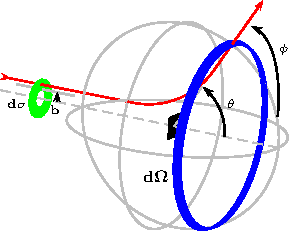
\includegraphics[width=0.8\textwidth]{./fig/sketch/compton_scattering_illustration_1.pdf}
    \caption{Showcase of solid angle $d\Omega$ and the differential size of the impact plane $d\sigma$ for $\theta=$~\unit{60}{deg}.}
    \label{fig:differential_cross_section_1}
  \end{subfigure}
  \begin{subfigure}{0.49\textwidth}
    \centering
    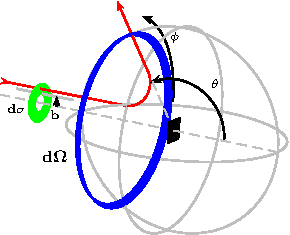
\includegraphics[width=0.8\textwidth]{./fig/sketch/compton_scattering_illustration_2.pdf}
    \caption{Showcase of solid angle $d\Omega$ and the differential size of the impact plane $d\sigma$ for $\theta=$~\unit{120}{deg}.}
    \label{fig:differential_cross_section_2}
  \end{subfigure}
  \caption{Illustration of the differential cross section for two possible values of $\theta$. The solid angle $d\Omega$ is integrated over all values of $\phi$ since the azimuthal angle $\phi$ is not changed by the scattering process.}
  \label{fig:differential_cross_section}
\end{figure}

Photon attenuation, i.e., the decrease of the intensity $d\Phi$ of an incident beam with original flux $\Phi \left[\mathrm{s}^{-1}\right]$ is described as
\begin{equation}
  \frac{d\Phi}{dz} = -n\sigma\Phi
\end{equation}
where $dz$ is the thickness of the blocking material, \unit{n_e}{\left[m^{-3}\right]} is the electron density of the material and $\sigma \left[\mathrm{m}^{2}\right]$ is the total cross section of the interaction.
By solving the differential equation, we obtain a relationship between the initial flux $\Phi$ and the remaining flux $\Phi_{out}$ behind the object with the thickness $z$:
\begin{equation}
  \Phi_{out} = \Phi e^{-n\sigma z}.
\end{equation}
This the probability of an \emph{event} (photoelectric effect, Compton scattering, etc.) $\mathrm{P}\left(E\right)$ is modeled as
\begin{equation}
  \mathrm{P}\left(E\right) = 1 - e^{-n\sigma z}.
\end{equation}

%%}

\subsection{Photoelectric effect}

%%{ Photoelectric effect

Photoelectric effect (Einstein, 1905) describes a total absorption of a photon by an electron.
When the electron is absorbed, the energy of the photon is completely consumed.
A portion of the energy is responsible for releasing the electron from the atomic orbital; the rest is converted to kinetic energy of the electron.

Photon energy can be expressed using its wavelength \unit{\lambda}{\left[m\right]} or frequency \unit{\nu}{\left[Hz\right]} as
\begin{equation}
  E_{\gamma} = \frac{hc}{\lambda} = h\nu,
\end{equation}
where $h \approx $ \unit{6.62 \cdot 10^{-34}}{m^2\,kg\,s^{-1}} is the Planck constant and \unit{c \approx 2.99 \cdot 10^{8}}{m\,s^{-1}} is the speed of light in a vacuum.
Let us define the ratio
\begin{equation}
  k = \frac{E_{\gamma}}{E_e}
\end{equation}
between the photon energy $E_{\gamma} = h\nu \left[\mathrm{eV}\right]$ and the electron rest mass energy \unit{E_e = m_ec^2 \approx 5.11 \cdot 10^5}{eV}.
According to \cite{fornalski2018simple}, the simplified version of the Gavrila-Pratt \cite{davisson1965interaction} cross section for the photoelectric effect is
\begin{equation}
  \label{eq:pe_cross_section}
  \sigma_{ph} = \frac{16}{3}\sqrt{2}\pi r_e^2\alpha^4\frac{Z^5}{k^{3.5}},
\end{equation}
where \unit{r_e \approx 2.81 \cdot 10^{-15}}{m} is the classical electron radius, $\alpha \approx 1/137.04$ is the fine structure constant and $Z$ is the atomic number of the element.
The accuracy of (\ref{eq:pe_cross_section}) is low even in the energy range, where it should be used ($\approx 1$ -- \unit{1000}{keV}).
To achieve better accuracy, one could build upon the work of, e.g., Gavrila-Pratt \cite{davisson1965interaction}, Scofield et al. \cite{scofield1973theoretical}, or Hubbell et al. \cite{hubbell1980pair}.
However, the cross section (\ref{eq:pe_cross_section}) will suffice for this work.

The probability of a single photoelectric effect event within a material of thickness $z$ is calculated as
\begin{equation}
  \mathrm{P}\left(E_{pe}\right) = 1 - e^{-n\sigma_{pe} z}.
\end{equation}

Cross section $\sigma_{ph}$ for $k > 0.9$
\begin{equation}
  \sigma_{ph} = Z^5\left[\sum_{n=1}^4 \frac{a_n + b_nZ}{1 + c_nZ}K^{-p_n}\right],
\end{equation}
where {\color{red} TODO } \cite{hubbell1980pair}.
\begin{table}
  \centering
  \begin{tabular}{c c c c c}
    \hline
    n & $a_n$ & $b_n$ & $c_n$ & $p_a$ \\
    \hline
    1 \rule{0pt}{2.3ex} & $1.6268 \cdot 10^{-9}$ & $-2.683 \cdot 10^{-12}$ & $4.173 \cdot 10^{-2}$ & 1 \\
    2 & $1.5274 \cdot 10^{-9}$ & $-5.110 \cdot 10^{-13}$ & $1.027 \cdot 10^{-2}$ & 2 \\
    3 & $1.1330 \cdot 10^{-9}$ & $-2.177 \cdot 10^{-12}$ & $2.013 \cdot 10^{-2}$ & 3.5 \\
    4 & $-9.12 \cdot 10^{-11}$ & 0 & 0 & 4\\
    \hline
  \end{tabular}
  \caption{\cite{hubbell1980pair}}
\end{table}

%%}

\subsection{Compton scattering}

%%{ Compton scattering

Compton scattering occurs when a photon transfers a portion of its energy to an electron.
During this interaction, the photon is deflected from its original path by the radial angle $\theta$ and azimuthal angle $\phi$.

The ratio $E_r$ of the energy of incoming ($E_{0}$) and scattered ($E_{s}$) particles was observed and described by Compton as
\begin{equation}
  E_r\left(\theta, E_0\right) = \frac{E_s\left(\theta, E_0\right)}{E_{0}} = \frac{1}{1 + \frac{E_0}{m_ec^2}\left(1 - \cos\theta\right)},
\end{equation}
where $\theta \in \left[-\pi, \pi\right)$ is the radial angle at which the photons are scattered, $E_0, E_s$ $\left[\mathrm{J}\right]$ are the energies of the incoming and scattered photons, \unit{m_e \approx 9.10 \cdot 10^{-31}}{kg} is the invariant mass of the electron, \unit{c \approx 2.99 \cdot 10^{8}}{m\,s^{-1}} is the speed of light in vacuum.

The Klein-Nishina formula \cite{leo2012techniques} describes the differential cross section \unit{d\sigma/d\Omega}{[m^2/sr]} of the incident and scattered beam as
\begin{equation}
  \label{eq:compton_differential_cross_section}
  \frac{d\sigma}{d\Omega}\left(\theta\right) = \frac{1}{2}\,r_{e}^2\,E_r\left(\theta\right)^2\left(E_r\left(\theta\right) + \frac{1}{E_r\left(\theta\right)} - \sin^2\theta\right),
\end{equation}
where \unit{r_e \approx 2.81 \cdot 10^{-15}}{m} is the classical electron radius.
As with the photoelectric effect, the prior probability of the scattering in a material with thickness $z$ is computed as:
\begin{equation}
  \label{eq:compton_prior}
  \mathrm{P}\left(E_{cs}\right) = 1 - e^{-n\sigma_{cs} z}.
\end{equation}
The value of likelihood probability density corresponding to the event $E_{cs}$ of a single photon with initial energy \unit{E_o}{[eV]} being scattered by the angle \unit{\theta}{[rad]} is calculated as
\begin{equation}
  \label{eq:compton_likelihood}
  \mathrm{P}\left(\theta \mid E_{cs}\right) = \frac{\int_0^{2\pi} \frac{d\sigma}{d\Omega}\,\sin \theta\,d\phi}{\sigma_{cs}},
\end{equation}
where $\sigma_{cs}$ is the total differential cross section for Compton scattering obtained from (\ref{eq:compton_differential_cross_section}).
To obtain the posterior probability density of the scattering under by the angle $\theta$, the likelihood (\ref{eq:compton_likelihood}) is multiplied by the prior probability of the Compton scattering (\ref{eq:compton_prior}):
\begin{equation}
  \mathrm{P}\left(E_{cs} \mid \theta\right) = \mathrm{P}\left(\theta \mid E_{cs}\right) \mathrm{P}\left(E_{cs}\right) = \left(1 - e^{-n\sigma_{cs} z}\right) \frac{\int_0^{2\pi} \frac{d\sigma}{d\Omega}\,\sin \theta\,d\phi}{\sigma_{cs}}.
\end{equation}

Figure~\ref{fig:compton_probs} shows the differential cross section of the Compton scattering, the likelihood of scattering by the angle $\theta$ and the posterior probability of scattering by the angle $\theta$, calculated for \unit{1}{mm} of silicon.

\begin{figure}[ht]
  \centering
  \begin{subfigure}{0.32\textwidth}
    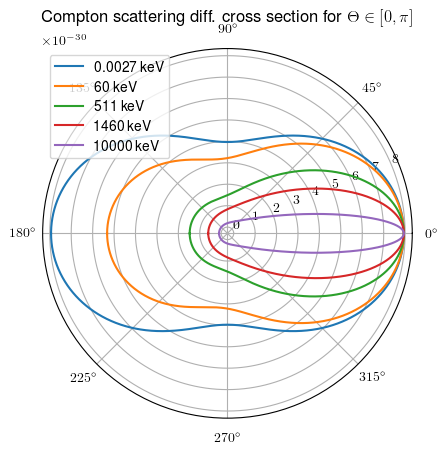
\includegraphics[width=1.0\textwidth]{./fig/klein_nishina_1.png}
    \caption{Plots of the differential cross $d\sigma/d\Omega$ section for various photon energies.}
    \label{fig:klein_1}
  \end{subfigure}
  \begin{subfigure}{0.32\textwidth}
    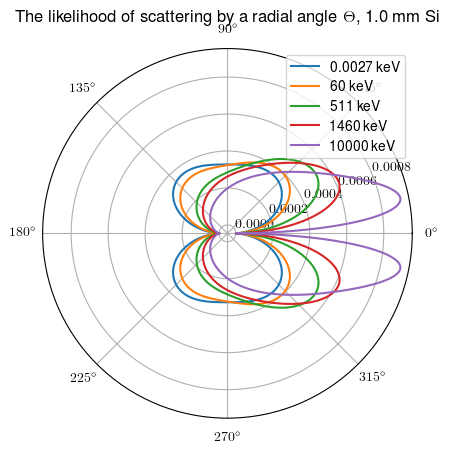
\includegraphics[width=1.0\textwidth]{./fig/klein_nishina_3.png}
    \caption{Plots of likelihood probability $\mathrm{P}\left(\theta \mid E_0\right)$, integrated over azimuthal angle $\phi$.}
    \label{fig:klein_2}
  \end{subfigure}
  \begin{subfigure}{0.32\textwidth}
    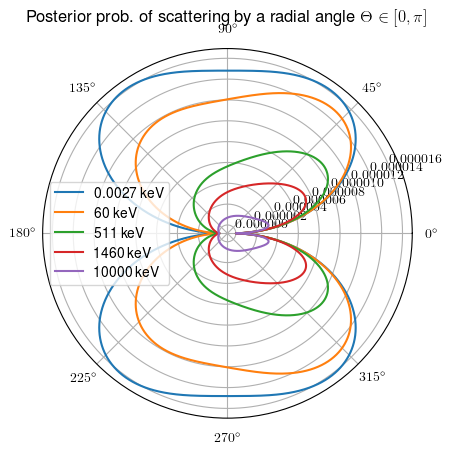
\includegraphics[width=1.0\textwidth]{./fig/klein_nishina_2.png}
    \caption{Plots of posterior probability $\mathrm{P}\left(E_0 \mid \theta\right)$, integrated over azimuthal angle $\phi$.}
    \label{fig:klein_3}
  \end{subfigure}
  \caption{Plots of the Klein-Nishina differential cross section (\ref{fig:klein_1}), the cross section normalized by the total cross section, integrate over the radial angle $\phi$ (\ref{fig:klein_2}) and the resulting probability distribution (\ref{fig:klein_3}), integrate over $\phi$.}
  \label{fig:compton_probs}
\end{figure}

% The intensity of the scattered beam \unit{N_s}{\left[s^{-1}\right]} is calculated for a small finite solid angle \unit{\Delta \theta}{\left[sr\right]} as
% \begin{equation}
%   N_s = N_o\,\frac{d\sigma}{d\Omega}\left(\theta\right)\,n_e\,t\,\Delta\theta,
% \end{equation}
% where \unit{N_0}{\left[s^{-1}\right]} is the intensity of the incoming beam, \unit{n_e}{\left[m^{-3}\right]} is the electron density of the scattering material and \unit{t}{\left[m\right]} is the effective thickness of the scattering material.

%%}

\subsection{Electron-positron pair and triplet production}

%%{ Electron-positron pair and triplet production

At higher energies, \unit{>1}{MeV}, the photoelectric effect and Compton scattering are dominated by the electron-positron pair and triplet productions effects \cite{hubbell1980pair}.
Since the aim of this work is to simulate the Compton camera, where only the first two effects are responsible in producing measurement, we omit the later two.
In the real sensor, the pair and triplet production would create an unwanted signal which would be filtered out by the processing software, responsible for particle track classification.

%%}

\subsection{Photon attenuation}

%%{ Photon attenuation

\begin{figure}[ht]
  \centering
  \begin{subfigure}{0.49\textwidth}
    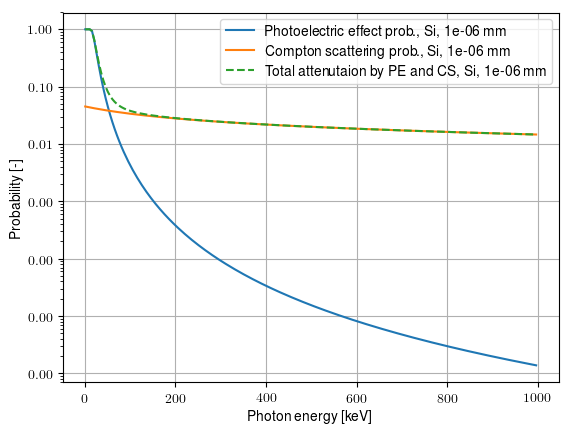
\includegraphics[width=1.0\textwidth]{./fig/scatterer_attenuation.png}
    \caption{Photon attenuation on \unit{1}{mm} of Si.}
    \label{fig:scatterer_attenuation}
  \end{subfigure}
  \begin{subfigure}{0.49\textwidth}
    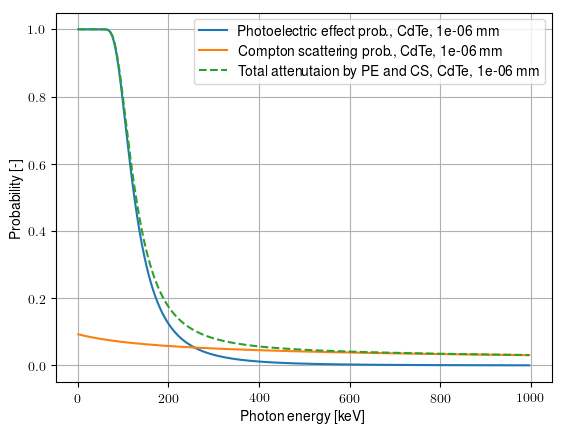
\includegraphics[width=1.0\textwidth]{./fig/absorber_attenuation.png}
    \caption{Photon attenuation on \unit{1}{mm} of CdTe.}
    \label{fig:absorber_attenuation}
  \end{subfigure}
  \label{fig:photon_attenuation}
  \caption{Photon attenuation on (\ref{fig:scatterer_attenuation}) the scatterer and (\ref{fig:absorber_attenuation}) the absorber.}
\end{figure}

%%}

%%}

\section{Compton camera principle}

\section{Gazebo/ROS camera model}

%%}

%% --------------------------------------------------------------
%% |  Chapter 8 - radiation source localization and estimation  |
%% --------------------------------------------------------------

\chapter{Radiation source state estimation}

%%{ Radiation source estimation

\section{The source direction hypotheses}

\subsection{Uncertainty propagation}

\section{Static case}

\section{Dynamic case}

\subsection{Assumptions}

\begin{itemize}
  \item A single radiation source,
  \item compact source,
  \item static,
  \item or moving with respect to a known model,
  \item ...
\end{itemize}

\subsection{2-D relaxation}

\subsection{General case}

%%}

%% --------------------------------------------------------------
%% |                   Chapter 9 - Evaluation                  |
%% --------------------------------------------------------------

\chapter{Evaluation}

%%{ Evaluation

\section{Simulation scenarios}

\section{``Traditional'' mapping with a scintillator}

\section{Micro Aerial Vehicle with the Compton camera}

\section{Group of Micro Aerial Vehicles with the Compton camera}

\section{Results}

%%}

%% --------------------------------------------------------------
%% |                  Chapter 10 - Conclusions                  |
%% --------------------------------------------------------------

\chapter{Conclusions}

%%{ Author's publications

Related journals (impacted):
\cite{baca2019autonomous}
\cite{baca2018rospix}
\cite{spurny2018cooperative}
\cite{saska2016system}
\cite{giernacky2019realtime}
\cite{chudoba2016exploration}

Related journals (unimpacted):
\cite{loianno2018localization}

Related conferences:
\cite{baca2019timepix}
\cite{baca2018model}
\cite{baca2016embedded}
\cite{baca2017autonomous}
\cite{saska2017documentation}
\cite{spurny2016complex}
\cite{faigl2017onsolution}
\cite{saska2016migrating}

Unrelated journals (impacted):
\cite{baca2016miniaturized}
\cite{baca2018vzlusat}
\cite{daniel2019inorbit}
\cite{urban2017vzlusat}

Unrelated conferences:
\cite{daniel2016terrestrial}
\cite{daniel2017xray}

%%}

%%{ REFERENCES

\conditionalClearPage
\printbibliography[notkeyword=mine]
\conditionalClearPage

%%}

%%{ APENDICES

\appendix
\renewcommand\chaptername{Appendix}

\chapter{List of author's publications}

Below are listed all publications of the author.
Each citation is displayed with percentage contribution of the author and number of citations based on Web of Science~(WoS), Scopus and Google Scholar~(GS).
Journal articles also contains information about the Impact Factor~(IF) by Web of Science and the CiteScore~(CS) by Scopus.
The publication~\cite{loianno2018localization} is only reported with CS due to the novelty of journal that is expected to receive impact factor in June 2020.

\section{Thesis-related author's publications}

\subsection*{Thesis-related articles in peer-reviewed journals with Impact Factor~(IF)}
\nocite{}
\printbibliography[keyword={mine},keyword={phd_related},keyword={journal},keyword={if},heading=none,title={}]

\subsection*{Thesis-related articles in peer-reviewed journals only with CiteScore~(CS)}
\nocite{}
\printbibliography[keyword={mine},keyword={phd_related},keyword={journal},keyword={cs},heading=none,title={}]

\subsection*{Thesis-related conference proceedings}
\nocite{}
\printbibliography[keyword={mine},keyword={phd_related},keyword={conference},heading=none,title={}]

\section{Thesis-unrelated author's publications}

\subsection*{Articles in peer-reviewed journals with impact factor}
\nocite{}
\printbibliography[keyword={mine},keyword={phd_unrelated},keyword={journal},keyword={if},heading=none,title={}]

\subsection*{Conference proceedings}
\nocite{}
\printbibliography[keyword={mine},keyword={phd_unrelated},keyword={conference},heading=none,title={}]

\appendix
\renewcommand\chaptername{Citations of author's work}

\chapter{Citations of author's work}

\DeclareCiteCommand{\fullcite}
{\usebibmacro{prenote}}
{\usedriver
  {\defcounter{minnames}{6}%
  \defcounter{maxnames}{6}}
{\thefield{entrytype}\clearfield{addendum}}}
{\multicitedelim}
{\usebibmacro{postnote}}

% \noindent
% \fullcite{baca2019autonomous}
% \begin{refsection}[citations/no_autocit/baca2019autonomous.bib]
%   \nocite{*}
%   \printbibliography[heading=none,title={},env=favoritebib]
% \end{refsection}

% \noindent
% \fullcite{spurny2018cooperative}
% \begin{refsection}[citations/no_autocit/spurny2018cooperative.bib]
%   \nocite{*}
%   \printbibliography[heading=none,title={},env=favoritebib]
% \end{refsection}

\noindent
\fullcite{saska2016system}
\begin{refsection}[citations/no_autocit/saska2016system.bib]
  \nocite{*}
  \printbibliography[heading=none,title={},env=favoritebib]
\end{refsection}

% \noindent
% \fullcite{giernacky2019realtime}
% \begin{refsection}[citations/no_autocit/giernacky2019realtime.bib]
%   \nocite{*}
%   \printbibliography[heading=none,title={},env=favoritebib]
% \end{refsection}

% \noindent
% \fullcite{chudoba2016exploration}
% \begin{refsection}[citations/no_autocit/chudoba2016exploration.bib]
%   \nocite{*}
%   \printbibliography[heading=none,title={},env=favoritebib]
% \end{refsection}

\noindent
\fullcite{loianno2018localization}
\begin{refsection}[citations/no_autocit/loianno2018localization.bib]
  \nocite{*}
  \printbibliography[heading=none,title={},env=favoritebib]
\end{refsection}

% \noindent
% \fullcite{baca2018model}
% \begin{refsection}[citations/no_autocit/baca2018model.bib]
%   \nocite{*}
%   \printbibliography[heading=none,title={},env=favoritebib]
% \end{refsection}

\noindent
\fullcite{baca2016embedded}
\begin{refsection}[citations/no_autocit/baca2016embedded.bib]
  \nocite{*}
  \printbibliography[heading=none,title={},env=favoritebib]
\end{refsection}

\noindent
\fullcite{baca2017autonomous}
\begin{refsection}[citations/no_autocit/baca2017autonomous.bib]
  \nocite{*}
  \printbibliography[heading=none,title={},env=favoritebib]
\end{refsection}

% \noindent
% \fullcite{saska2017documentation}
% \begin{refsection}[citations/no_autocit/saska2017documentation.bib]
%   \nocite{*}
%   \printbibliography[heading=none,title={},env=favoritebib]
% \end{refsection}

% \noindent
% \fullcite{spurny2016complex}
% \begin{refsection}[citations/no_autocit/spurny2016complex.bib]
%   \nocite{*}
%   \printbibliography[heading=none,title={},env=favoritebib]
% \end{refsection}

% \noindent
% \fullcite{faigl2017onsolution}
% \begin{refsection}[citations/no_autocit/faigl2017onsolution.bib]
%   \nocite{*}
%   \printbibliography[heading=none,title={},env=favoritebib]
% \end{refsection}

% \noindent
% \fullcite{saska2016migrating}
% \begin{refsection}[citations/no_autocit/saska2016migrating.bib]
%   \nocite{*}
%   \printbibliography[heading=none,title={},env=favoritebib]
% \end{refsection}

\noindent
\fullcite{baca2016miniaturized}
\begin{refsection}[citations/no_autocit/baca2016miniaturized.bib]
  \nocite{*}
  \printbibliography[heading=none,title={},env=favoritebib]
\end{refsection}

\noindent
\fullcite{urban2017vzlusat}
\begin{refsection}[citations/no_autocit/urban2017vzlusat.bib]
  \nocite{*}
  \printbibliography[heading=none,title={},env=favoritebib]
\end{refsection}

\noindent
\fullcite{daniel2016terrestrial}
\begin{refsection}[citations/no_autocit/daniel2016terrestrial.bib]
  \nocite{*}
  \printbibliography[heading=none,title={},env=favoritebib]
\end{refsection}

\noindent
\fullcite{daniel2017xray}
\begin{refsection}[citations/no_autocit/daniel2017xray.bib]
  \nocite{*}
  \printbibliography[heading=none,title={},env=favoritebib]
\end{refsection}

%%}

\end{document}
